\section{Signal modelling}

The parameterization based on simulated samples of \mfl distributions for signals are described in this section.
Several signal models are studied in this analysis, including heavy Higgs like narrow-width signal (NWA) and large-width signal (LWA), as well as the modelling of Randall-Sundrum graviton (RSG) signal.

\subsection{Modelling of narrow-width signal}

For narrow-width signal, the \mfl width is totally determined by detector resolution, which is modelled 
by the sum of a Crystal Ball ($\mathcal{C}$) function~\cite{CrystalBall1,CrystalBall2} and a Gaussian ($\mathcal{G}$) function:

\begin{equation}
    \label{eq:cb_plus_g}
    P_{s} (\mfl) = f_{\mathcal{C}} \cdot \mathcal{C}(\mfl; \mu, \sigma_{\mathcal{C}}, \alpha_{\mathcal{C}}, n_{\mathcal{C}})
                   + (1 - f_{\mathcal{C}}) \cdot \mathcal{G}(\mfl; \mu, \sigma_{\mathcal{G}})
\end{equation}

The two functions share the same central value $\mu$, while the resolution parameters, $\sigma_{\mathcal{C}}$ and $\sigma_{\mathcal{G}}$, are different.
In the Crystal Ball function, the parameters $\alpha_{\mathcal{C}}$ and $n_{\mathcal{C}}$ model the shape of non-Gaussian tail,
and the fraction parameter $f_{\mathcal{C}}$ is used to ensure the relative normalization between two functions.

The parameters are obtained by fitting to signal MC simulations combining the mc16a, mc16d and mc16e campaigns for each category separately at each mass points from 200~\gev to 2000~\gev,
and the shape of ggF and VBF signals are found to be similar.
Figure~\ref{fig:ggf_mass_signalParam_2mu2e} shows the \mfl distribution and fitted curves for ggF production at mass from 200~\gev to 2000~\gev in 2$e$2$\mu$ channel as examples.

\begin{figure}[htbp]
    \centering
    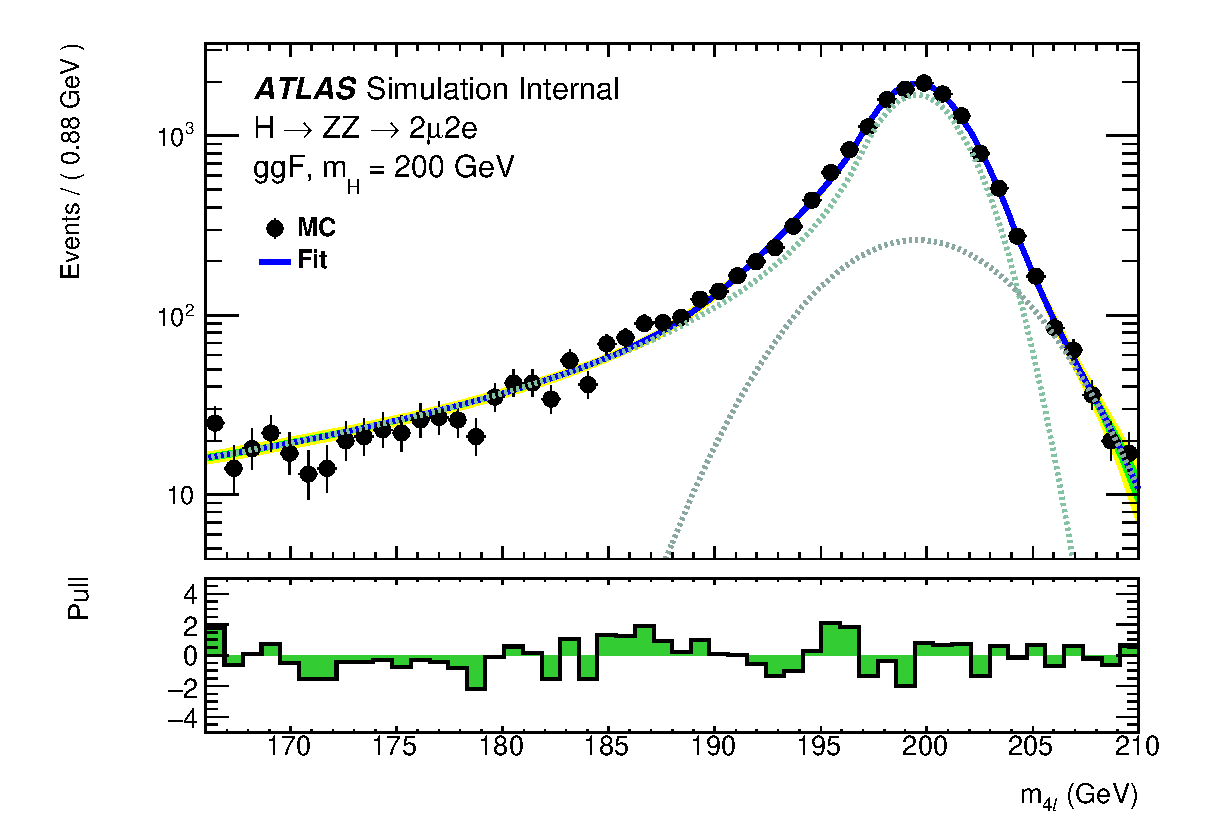
\includegraphics[width=0.32\textwidth]{figures/HMHZZ/signal/ggf_mass_signal_200_H4l_2mu2e.eps}
    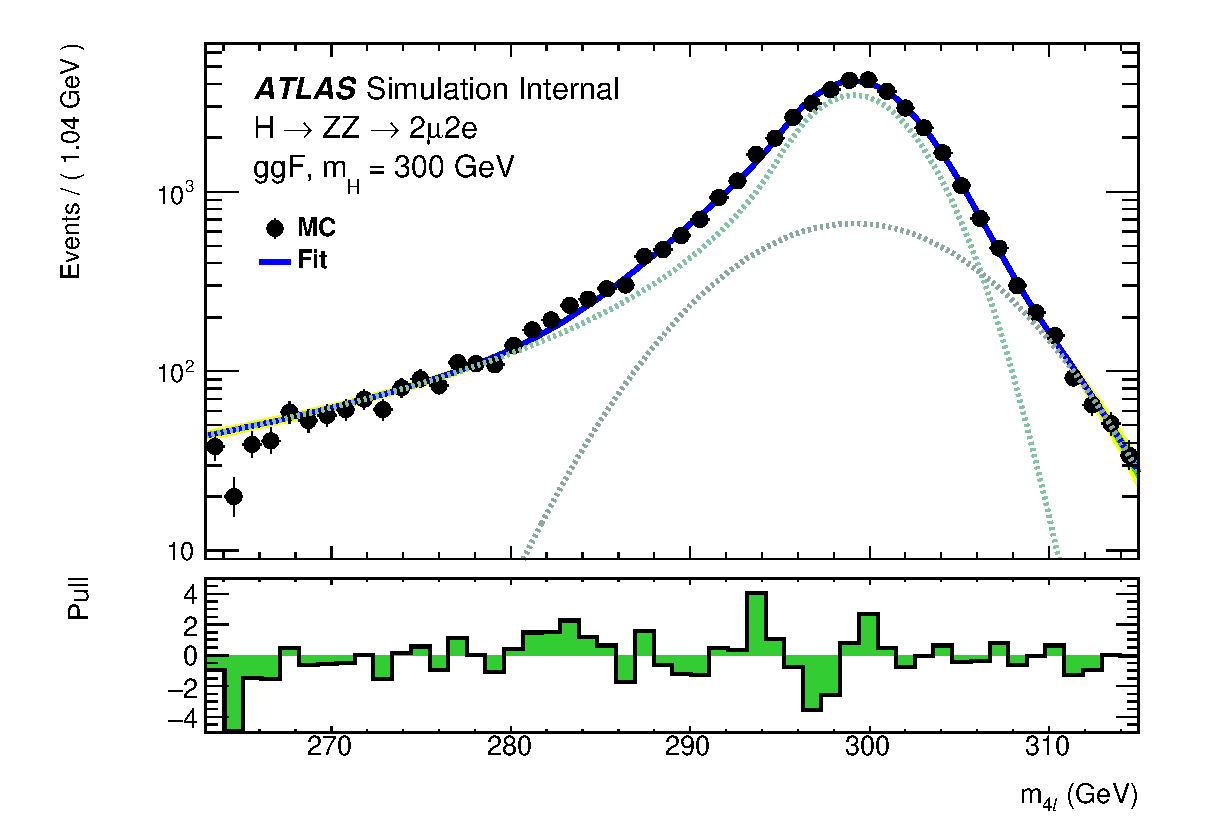
\includegraphics[width=0.32\textwidth]{figures/HMHZZ/signal/ggf_mass_signal_300_H4l_2mu2e.eps}
    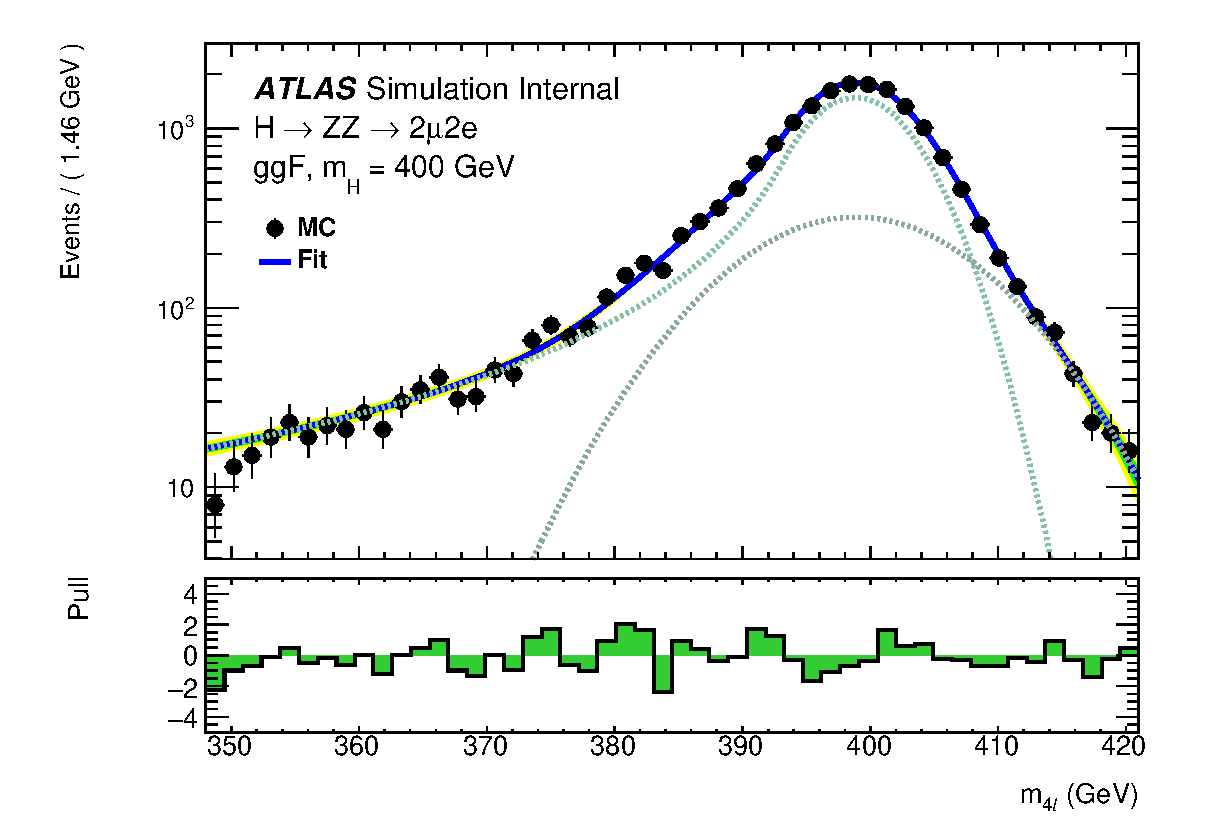
\includegraphics[width=0.32\textwidth]{figures/HMHZZ/signal/ggf_mass_signal_400_H4l_2mu2e.eps}\\
    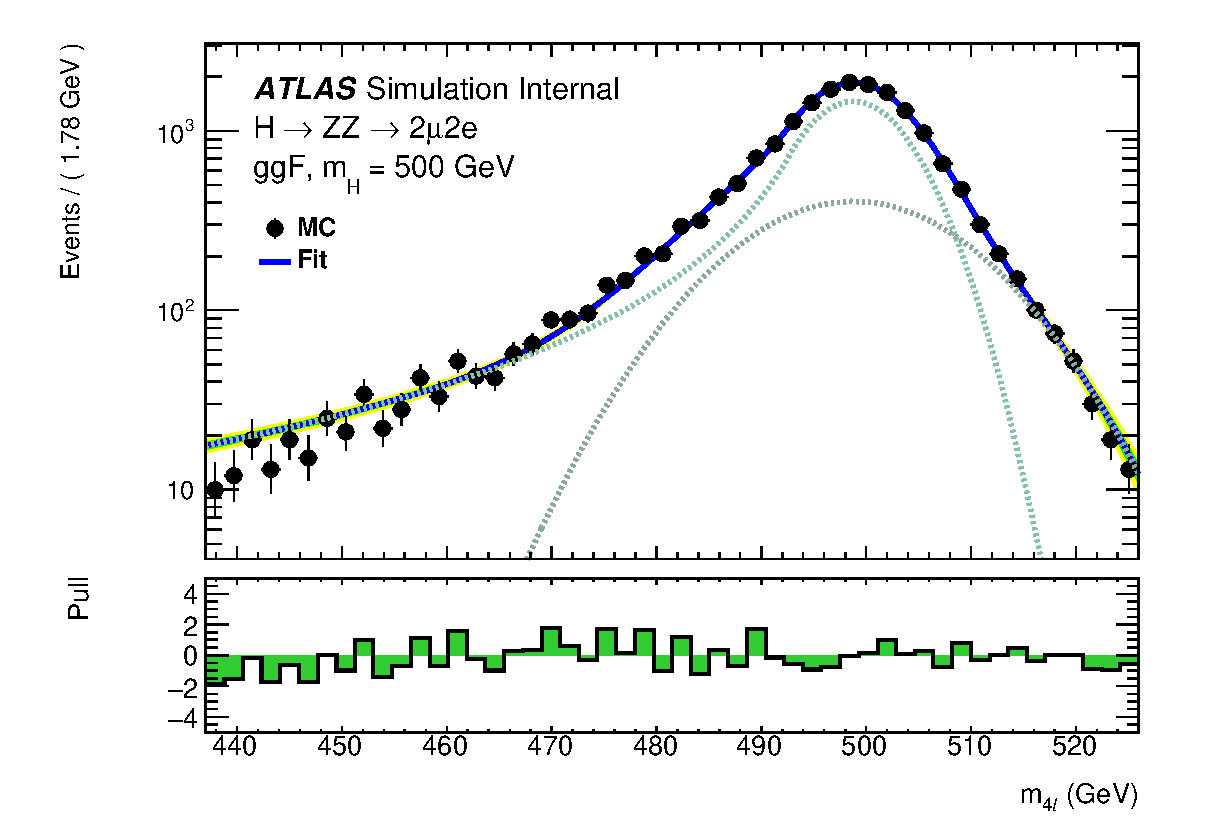
\includegraphics[width=0.32\textwidth]{figures/HMHZZ/signal/ggf_mass_signal_500_H4l_2mu2e.eps}
    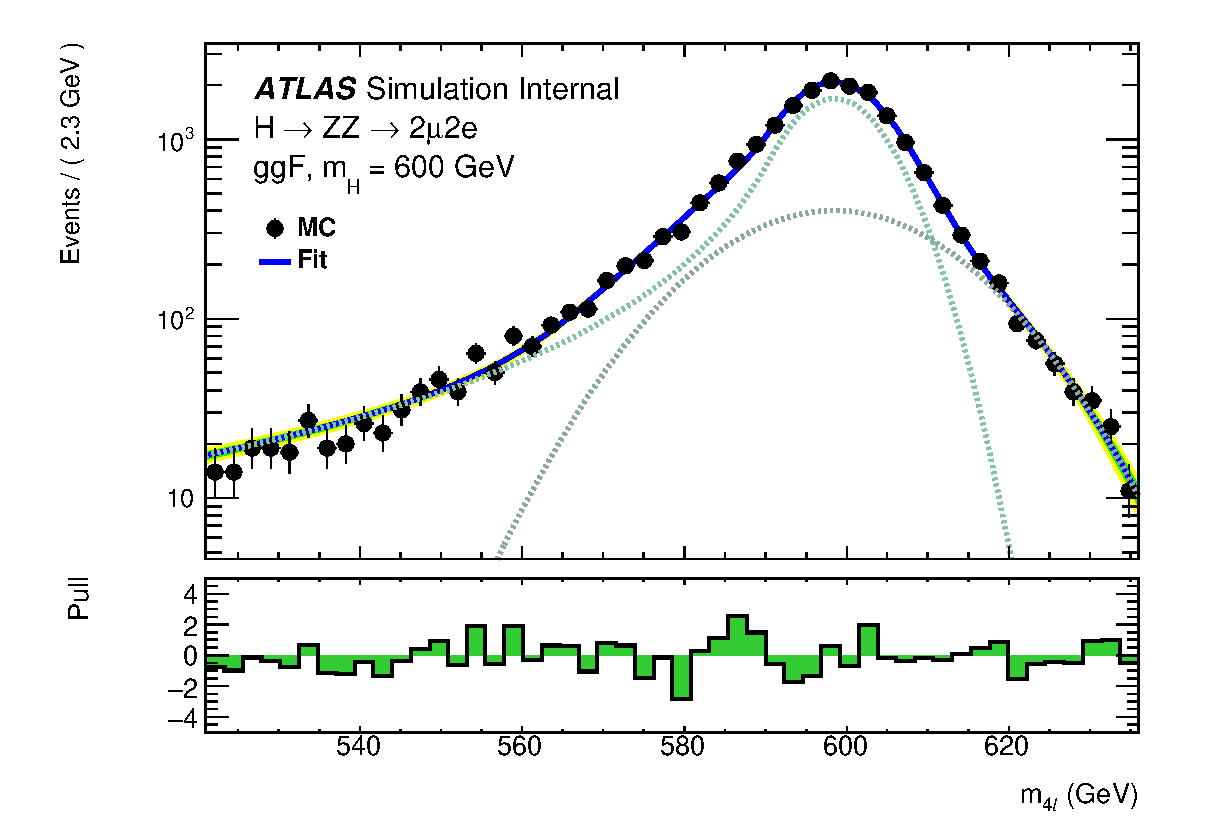
\includegraphics[width=0.32\textwidth]{figures/HMHZZ/signal/ggf_mass_signal_600_H4l_2mu2e.eps}
    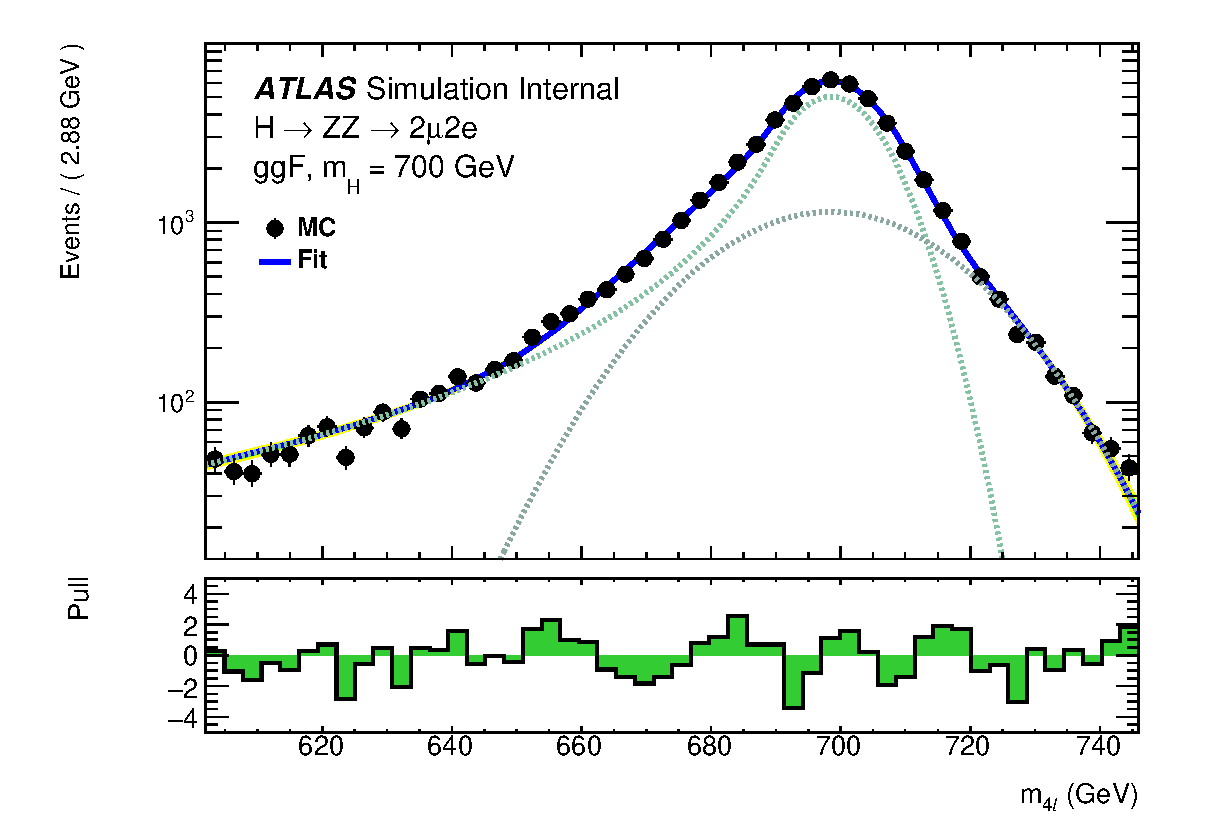
\includegraphics[width=0.32\textwidth]{figures/HMHZZ/signal/ggf_mass_signal_700_H4l_2mu2e.eps}\\
    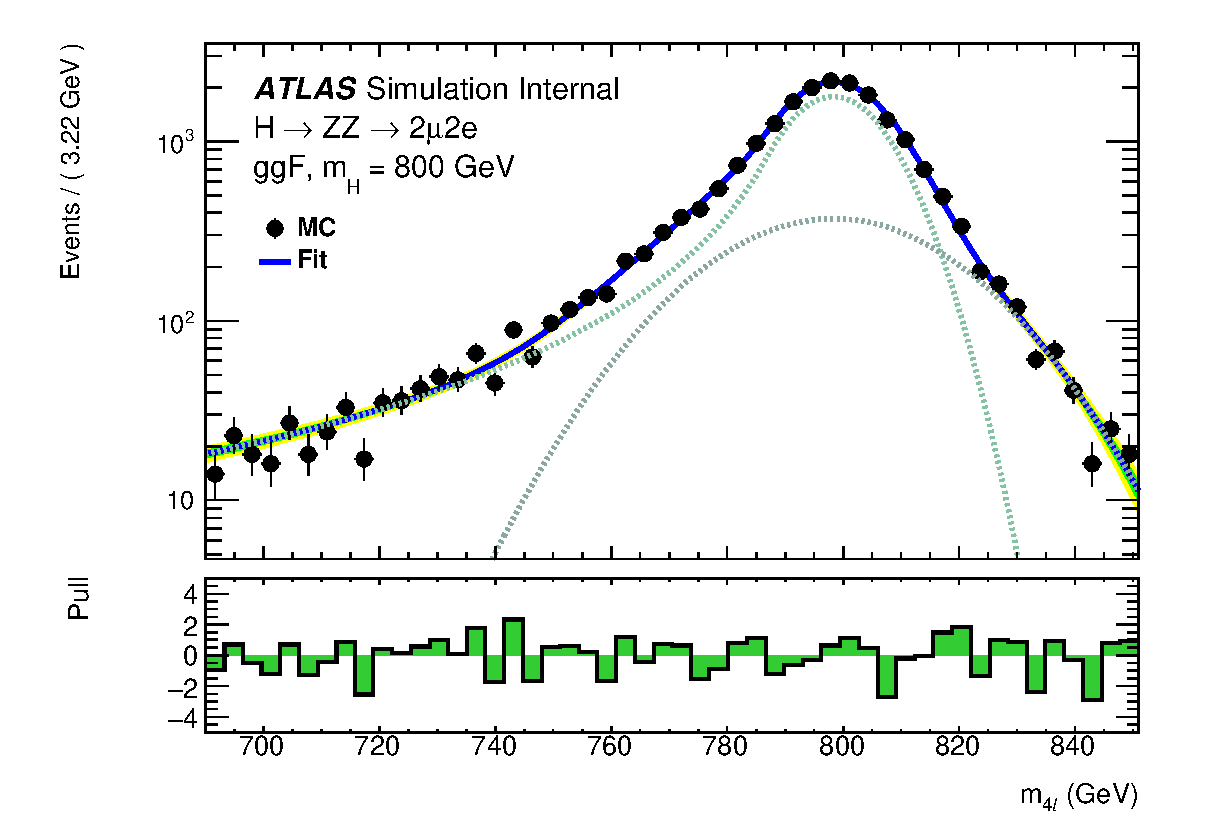
\includegraphics[width=0.32\textwidth]{figures/HMHZZ/signal/ggf_mass_signal_800_H4l_2mu2e.eps}
    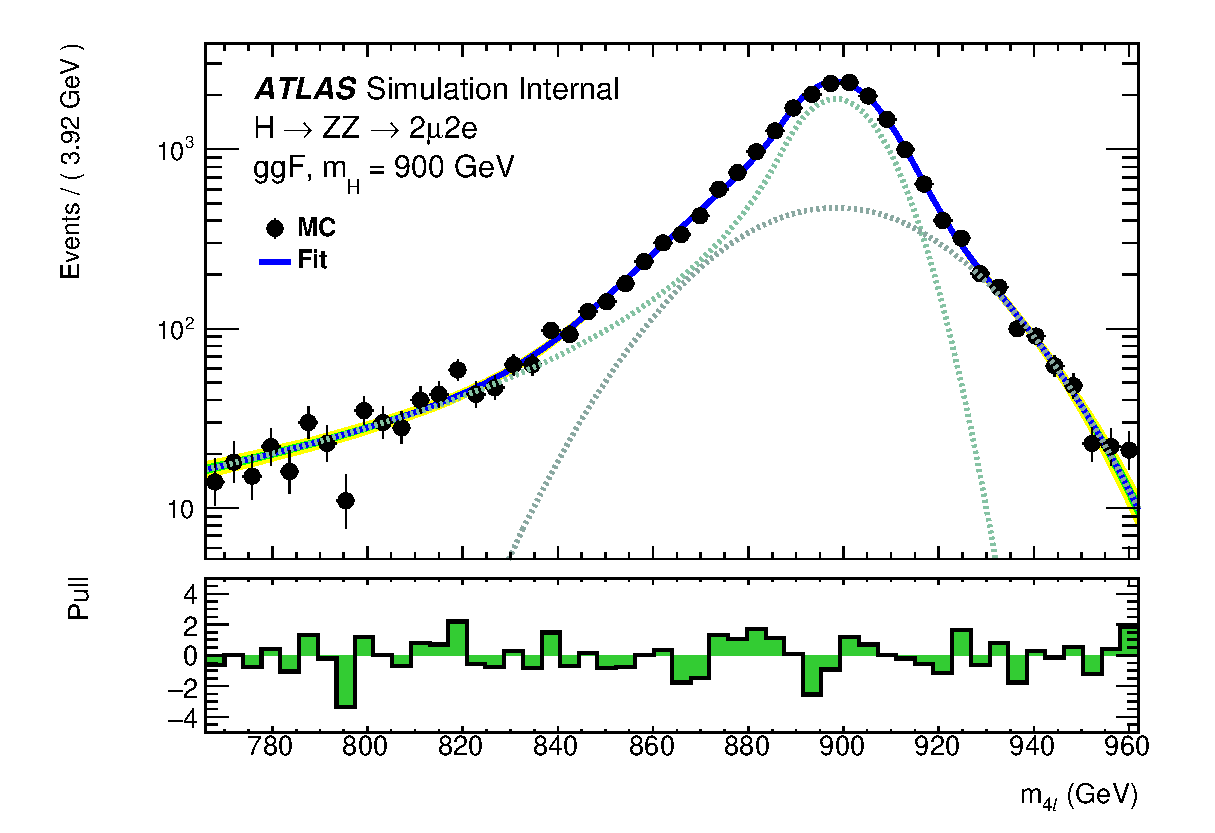
\includegraphics[width=0.32\textwidth]{figures/HMHZZ/signal/ggf_mass_signal_900_H4l_2mu2e.eps}
    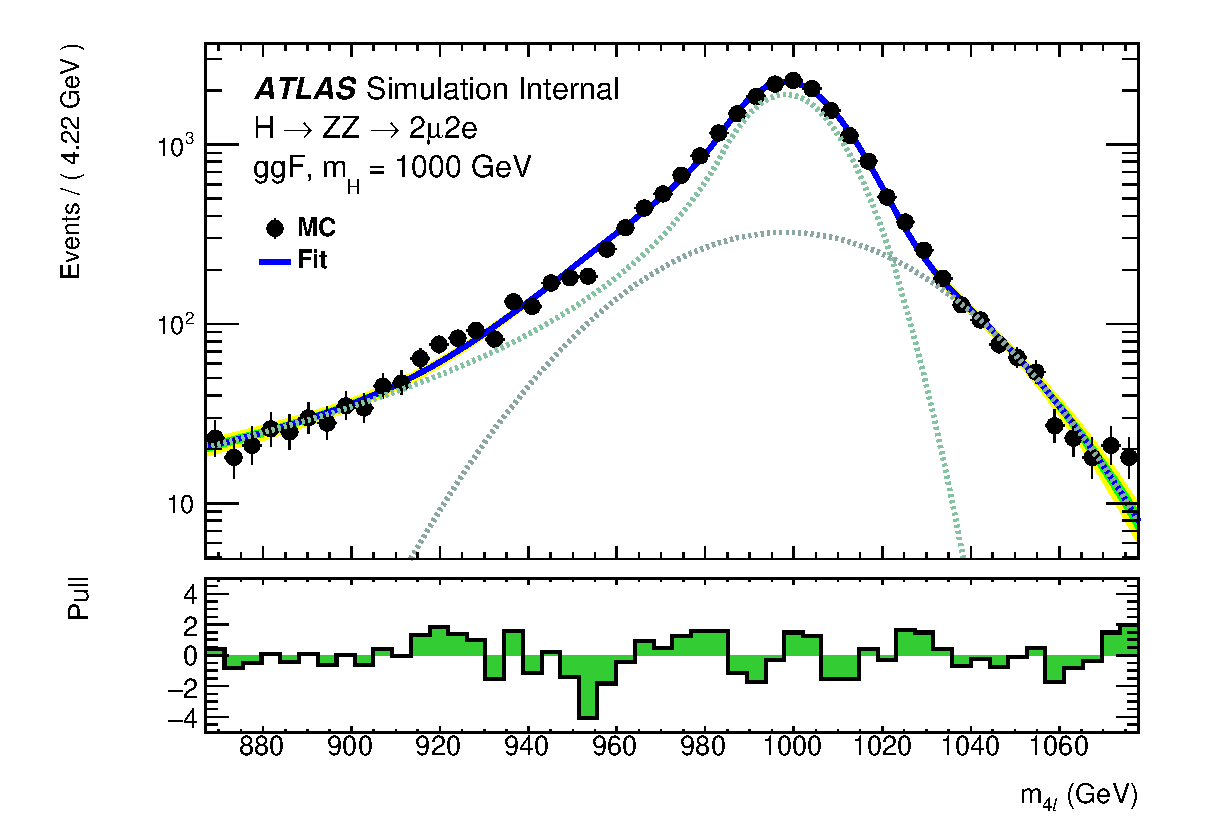
\includegraphics[width=0.32\textwidth]{figures/HMHZZ/signal/ggf_mass_signal_1000_H4l_2mu2e.eps}\\
    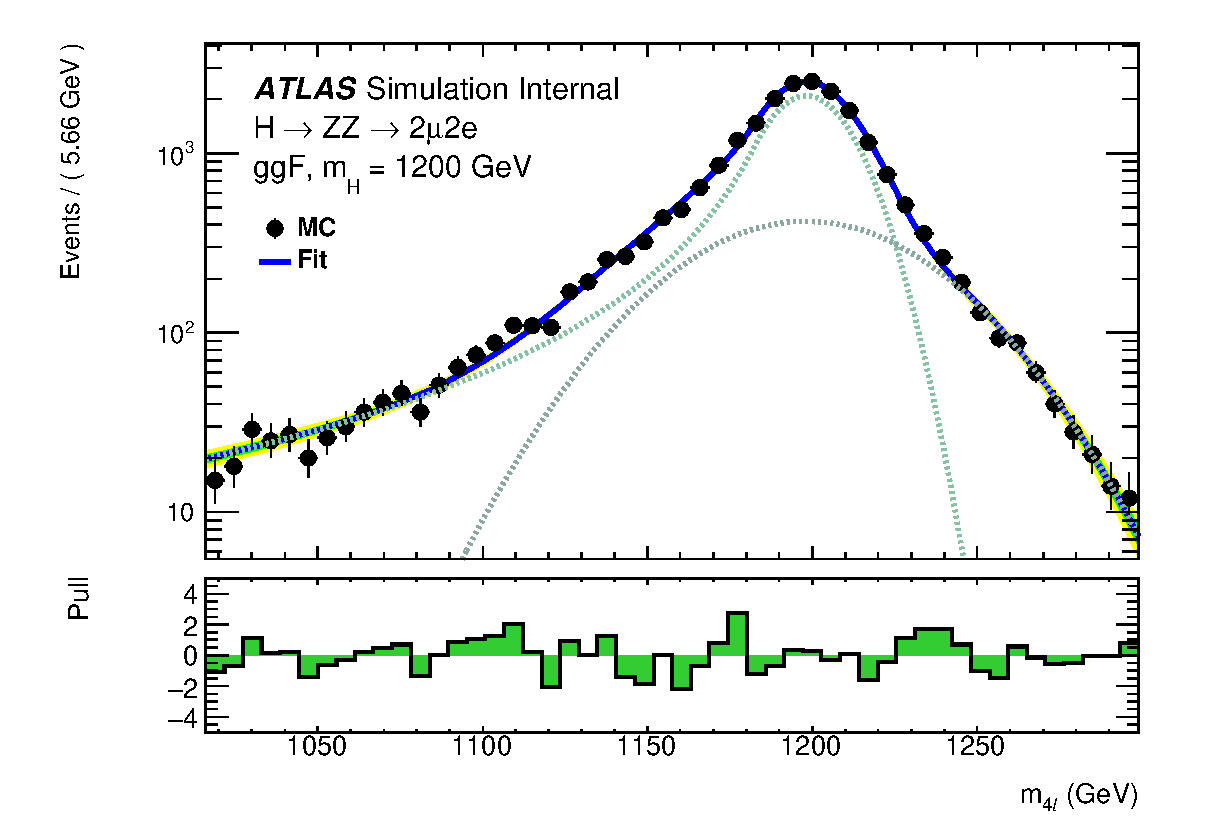
\includegraphics[width=0.32\textwidth]{figures/HMHZZ/signal/ggf_mass_signal_1200_H4l_2mu2e.eps}
    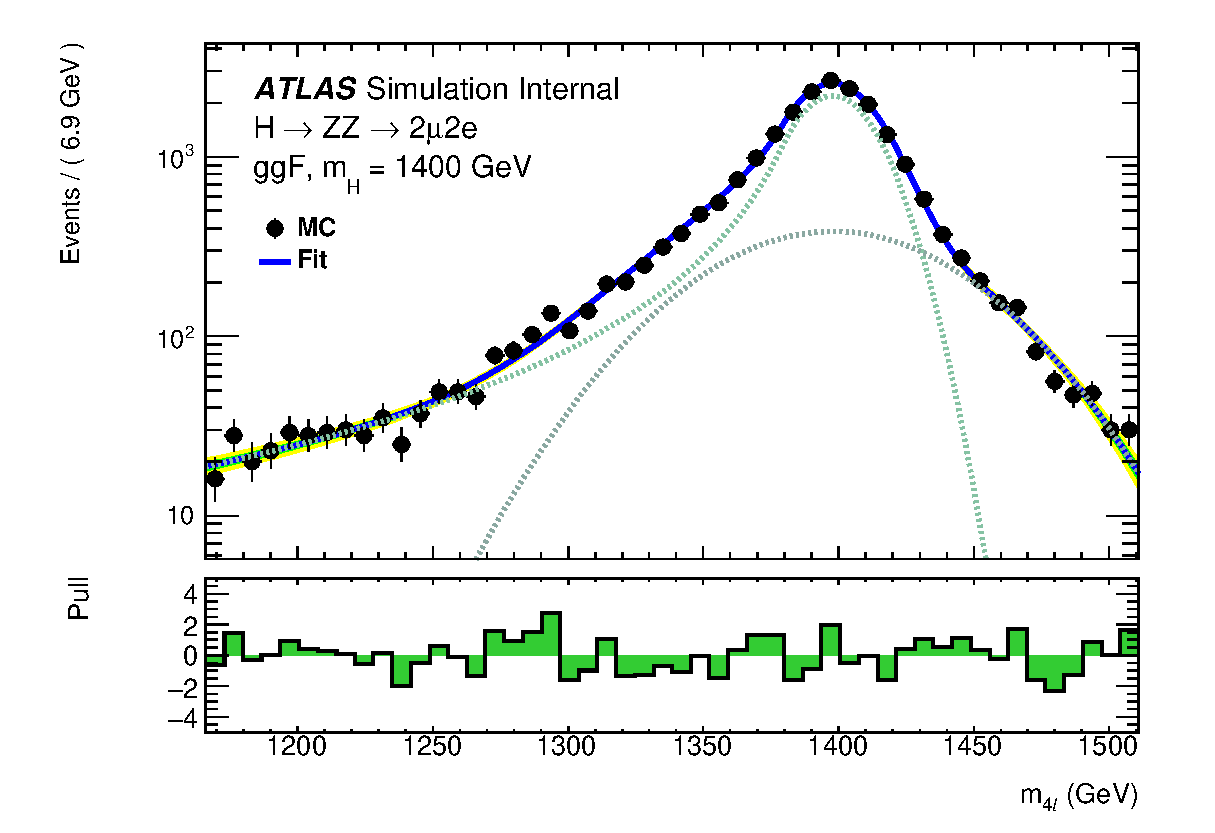
\includegraphics[width=0.32\textwidth]{figures/HMHZZ/signal/ggf_mass_signal_1400_H4l_2mu2e.eps}
    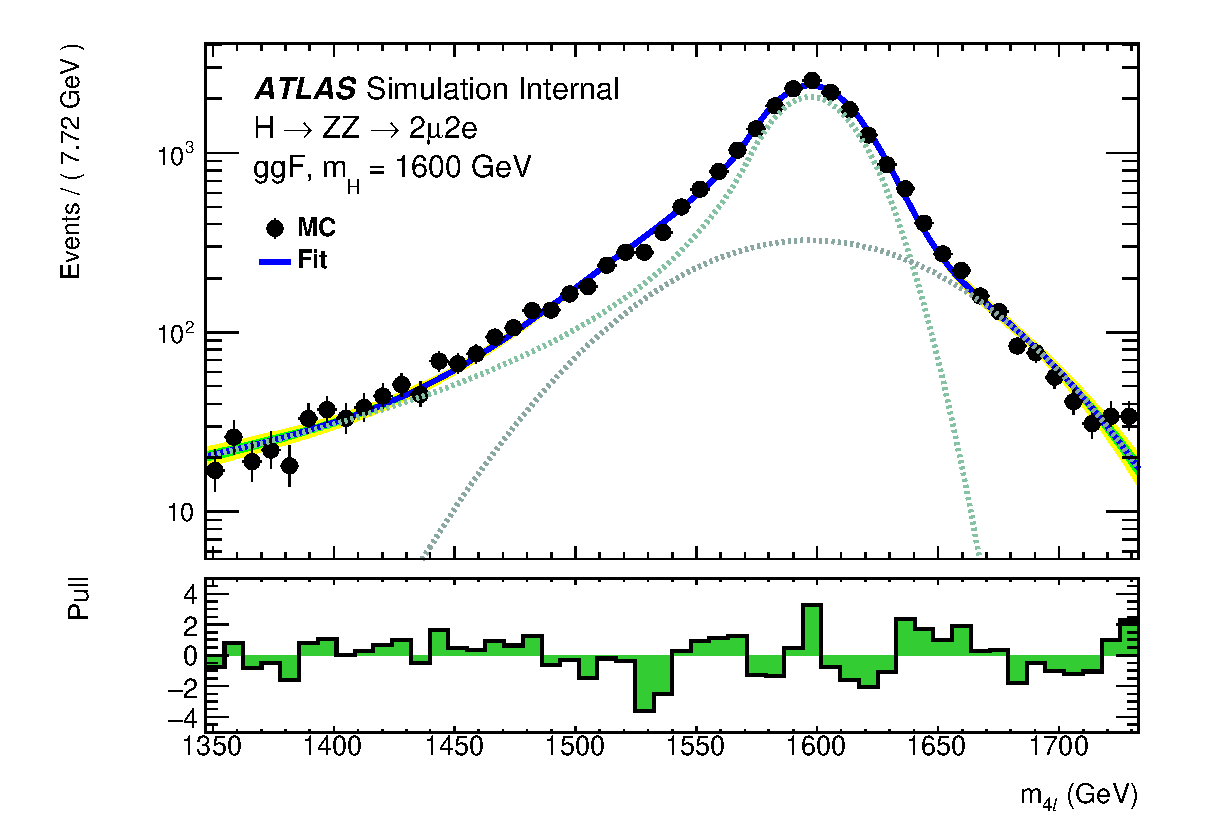
\includegraphics[width=0.32\textwidth]{figures/HMHZZ/signal/ggf_mass_signal_1600_H4l_2mu2e.eps}\\
    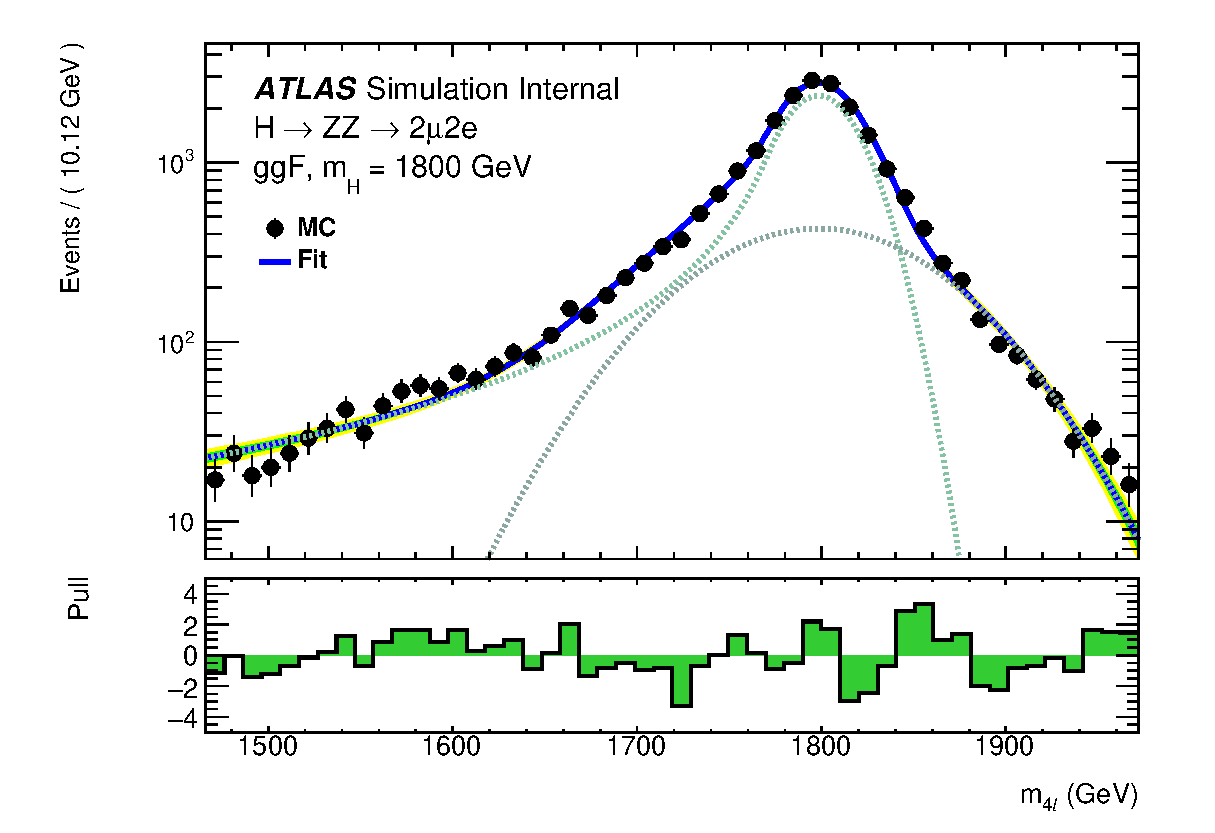
\includegraphics[width=0.32\textwidth]{figures/HMHZZ/signal/ggf_mass_signal_1800_H4l_2mu2e.eps}
    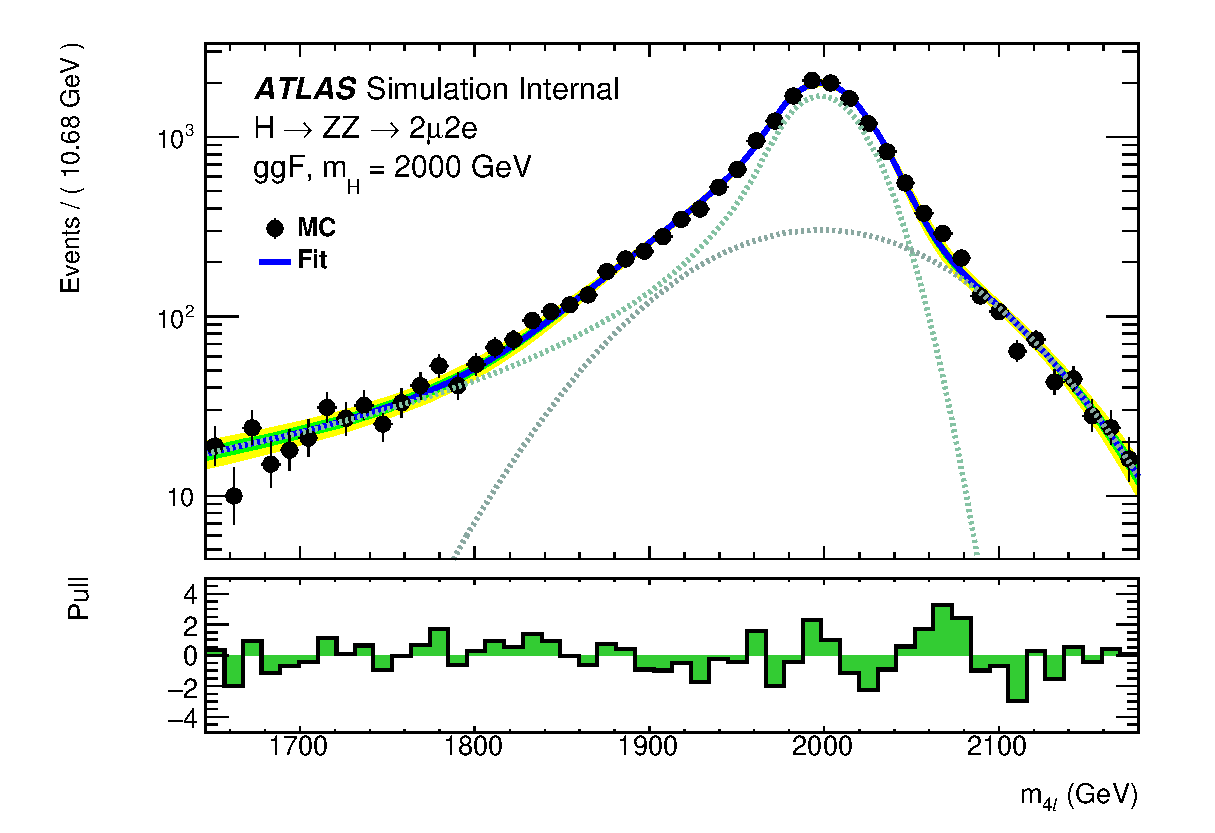
\includegraphics[width=0.32\textwidth]{figures/HMHZZ/signal/ggf_mass_signal_2000_H4l_2mu2e.eps}
    \caption{Distributions of the $m_{2\mu 2e}$ and fit projection for signal samples between 200 to 3000~\gev for ggF production mode. 
    Three MC campaigns, mc16a, mc16d and mc16e, are combined. 
    The lower panel in each plot shows the pull distribution.}
    \label{fig:ggf_mass_signalParam_2mu2e}
\end{figure}

Then the $\mathcal{C}+\mathcal{G}$ parameters are fitted with a polynomial as functions of generated mass points (\mH) for samples, as an example shown in figure~\ref{fig:ggf_fitParams_interpolation_2mu2e} for 2$e$2$\mu$ channel.
The fitting quality can be measured by the Pearson’s $\chi^2$, which is within 3 (2) for 2$e$2$\mu$ (4$e$ and 4$\mu$) channel.

\begin{figure}[htbp]
    \centering
    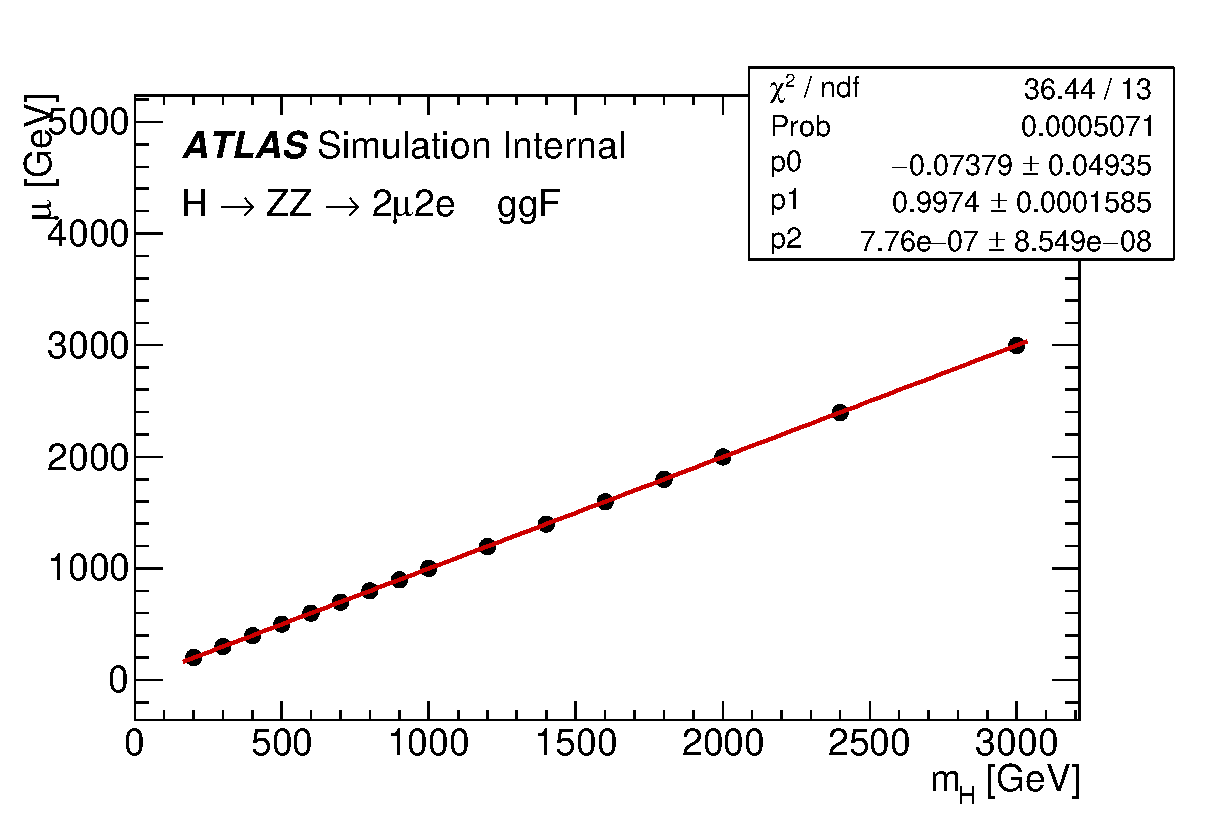
\includegraphics[width=0.32\textwidth]{figures/HMHZZ/signal/ggf_graph_mass_mean_2mu2e_fit.eps}
    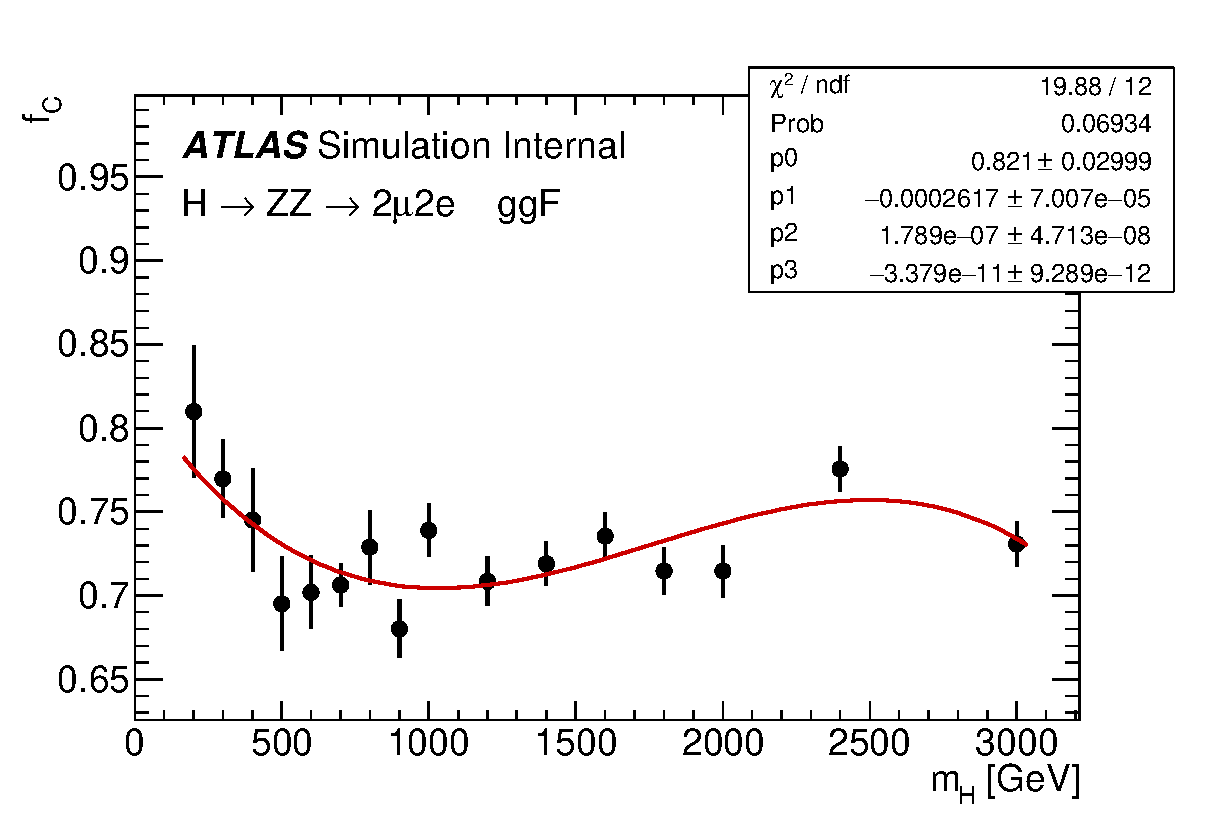
\includegraphics[width=0.32\textwidth]{figures/HMHZZ/signal/ggf_graph_f_cb_gauss_2mu2e_fit.eps}
    \includegraphics[width=0.32\textwidth]{figures/HMHZZ/signal/ggf_graph_mass_gauss_sigma_2mu2e_fit.eps} \\
    \includegraphics[width=0.32\textwidth]{figures/HMHZZ/signal/ggf_graph_mass_cb_sigma_2mu2e_fit.eps}
    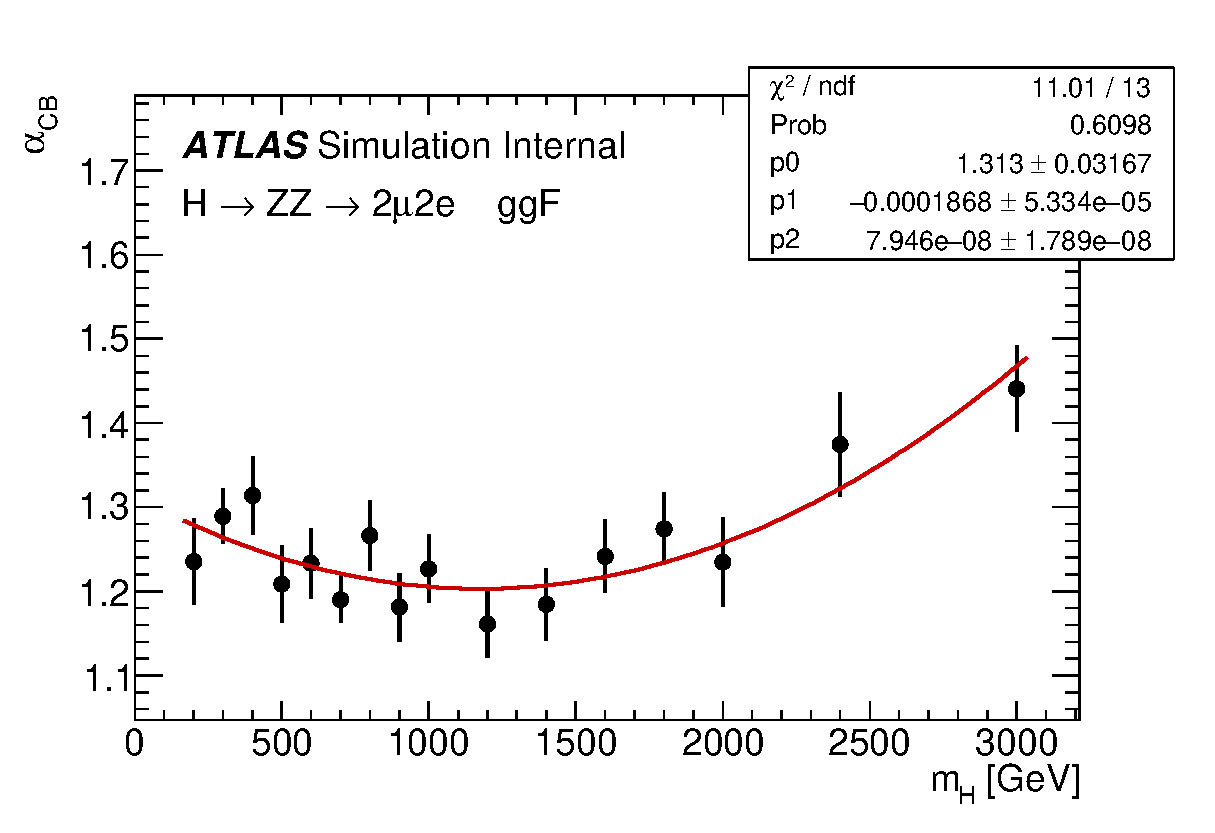
\includegraphics[width=0.32\textwidth]{figures/HMHZZ/signal/ggf_graph_mass_cb_alpha_2mu2e_fit.eps}
    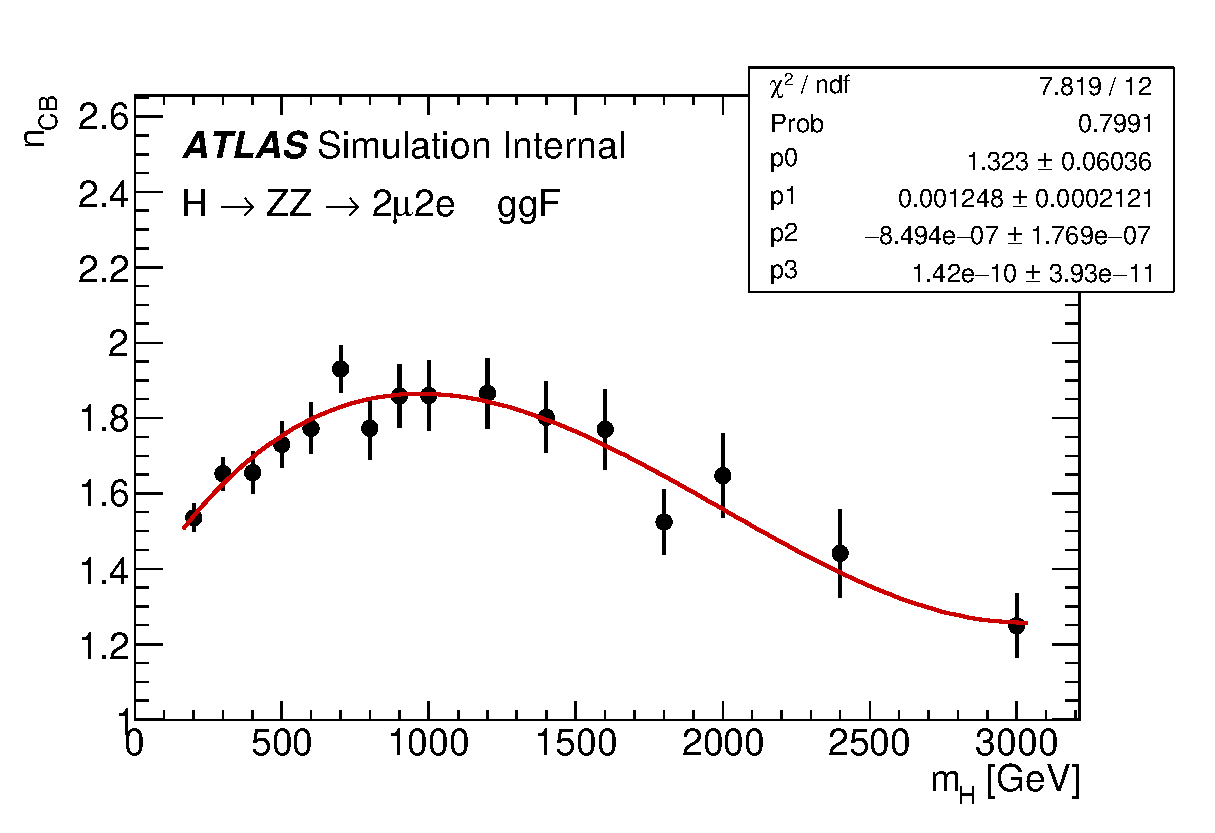
\includegraphics[width=0.32\textwidth]{figures/HMHZZ/signal/ggf_graph_mass_cb_n_2mu2e_fit.eps}
    \caption{Polynomial fits of the parameters $\mu$, $f_{\mathcal{C}}$, $\sigma_{\mathcal{G}}$, $\sigma_{\mathcal{C}}$,
    $n_{\mathcal{C}}$ and $\alpha_{\mathcal{C}}$ for the signal $\mathcal{C}+\mathcal{G}$ model in the $2\mu 2e$ channel as a function of \mH for
    the ggF production mode. The combination of the mc16a, mc16d and mc16e MC campaigns is used.}
    \label{fig:ggf_fitParams_interpolation_2mu2e}
\end{figure}

In addition, possible difference on the signal yield extracted from parameterization and MC simulation is studied.
Figure~\ref{fig:ggf_graph_YieldCheckAll} shows this difference by computing $\frac{N_{\text{reco}}-N_{\text{fit}}}{N_{\text{fit}}}$, where $N_{\text{reco}}$ denotes the total number of reconstructed events observed from MC simulation at that mass point
and $N_{\text{fit}}$ depicts the number of events obtained from the fitted PDF.
The differences are treated as an additional systematic uncertainty with the value of 2\% (1\%) for 2$e$2$\mu$ (4$e$ and 4$\mu$) channel in the analysis.

\begin{figure}[htbp]
    \centering
    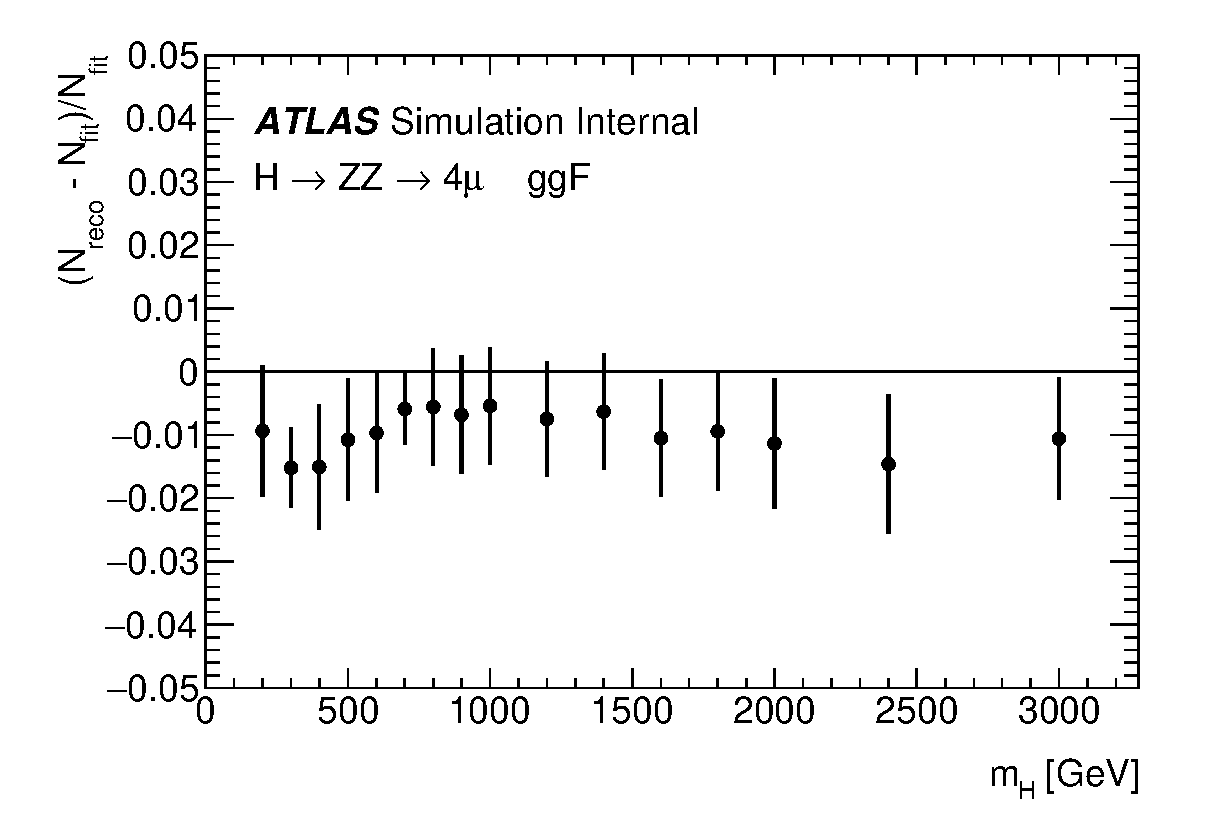
\includegraphics[width=0.32\textwidth]{figures/HMHZZ/signal/ggf_graph_YieldCheck_4mu_fixed.eps}
    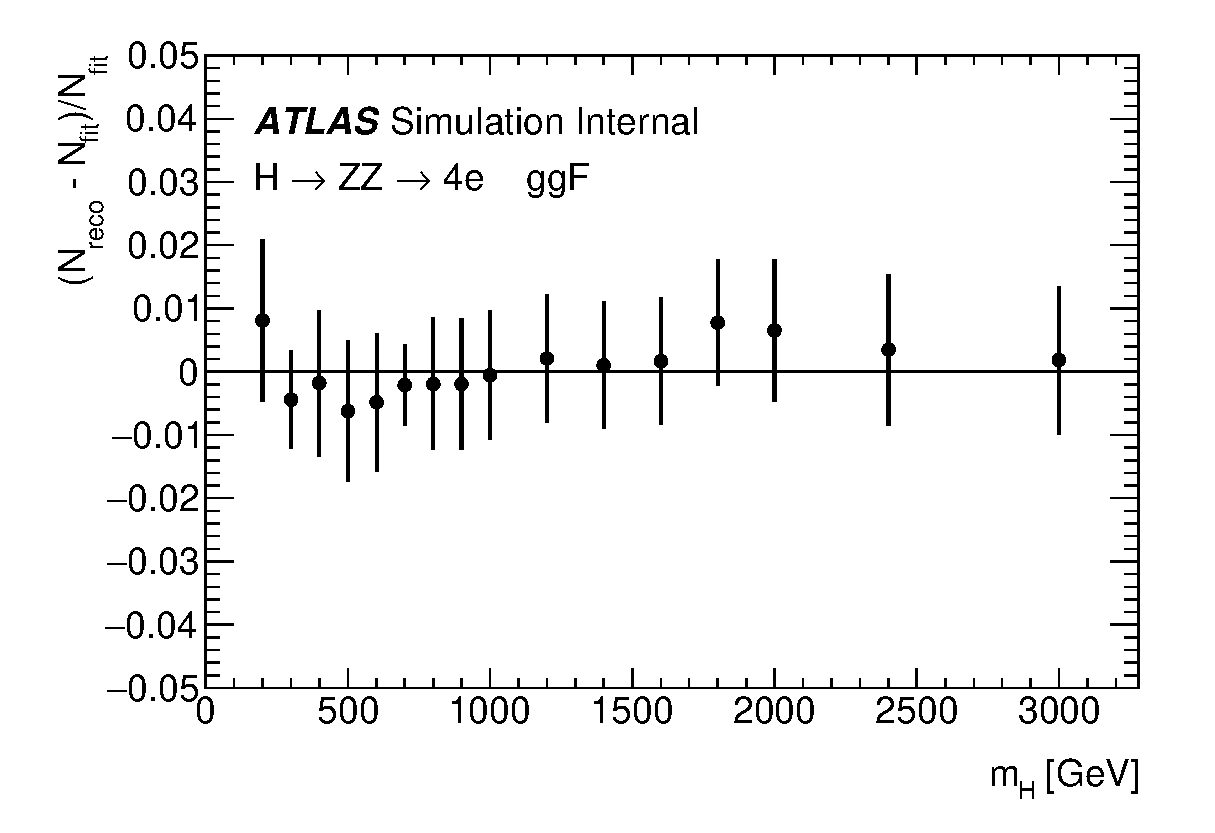
\includegraphics[width=0.32\textwidth]{figures/HMHZZ/signal/ggf_graph_YieldCheck_4e_fixed.eps}
    \includegraphics[width=0.32\textwidth]{figures/HMHZZ/signal/ggf_graph_YieldCheck_2mu2e_fixed.eps}
    \caption{The difference between MC simulation and parameterization of
    $4\mu$ (left), $4e$ (middle) and $2\mu 2e$ (right) for the ggF production
    mode. The combination of the mc16a, mc16d and mc16e MC campaigns is used.}
    \label{fig:ggf_graph_YieldCheckAll}
\end{figure}

In summary, the final interpolated signal shapes for the ggF production mode are shown together in figure~\ref{fig:ggf_multipeak} for mass points with step of 100~\gev from 200~\gev to 3000~\gev.

\begin{figure}[htbp]
    \centering
    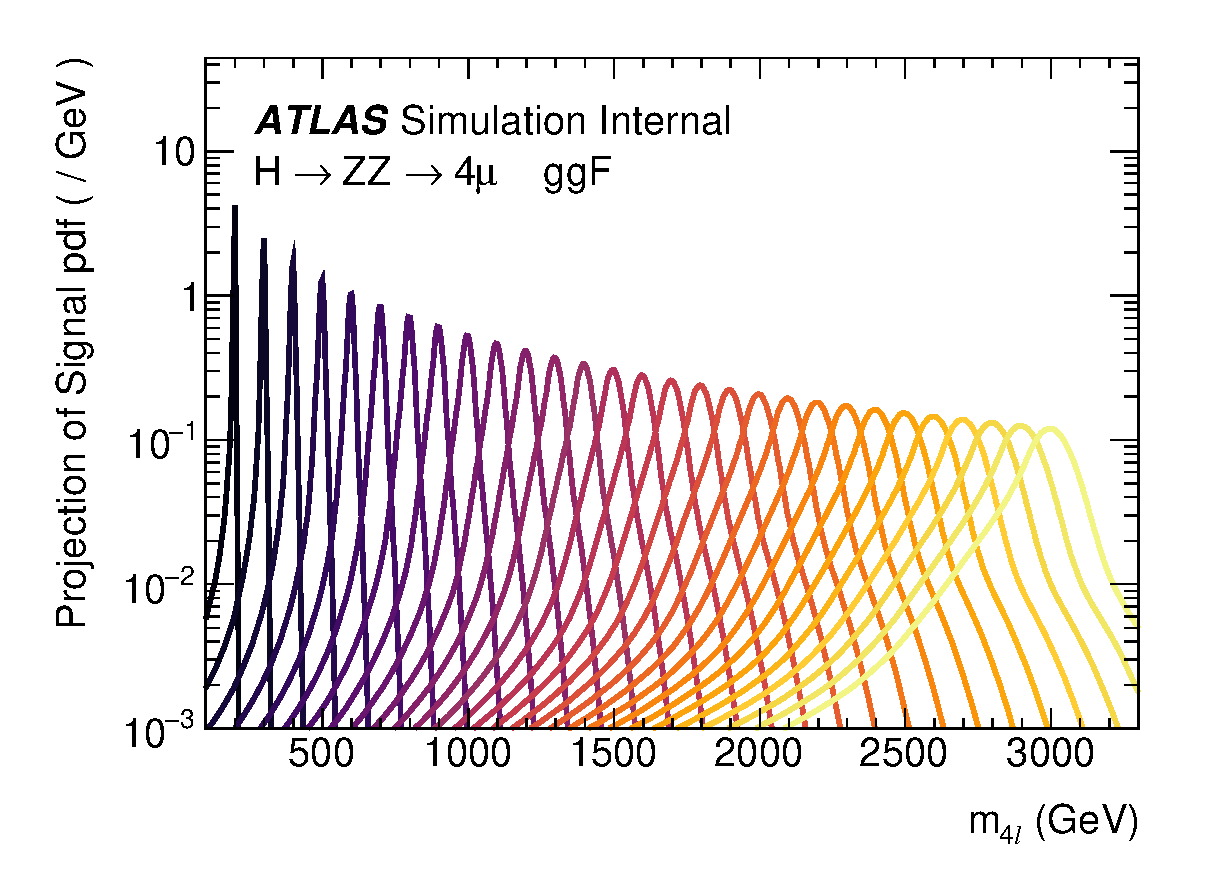
\includegraphics[width=0.32\textwidth]{figures/HMHZZ/signal/ggf_multipeakplot_4mu.eps}
    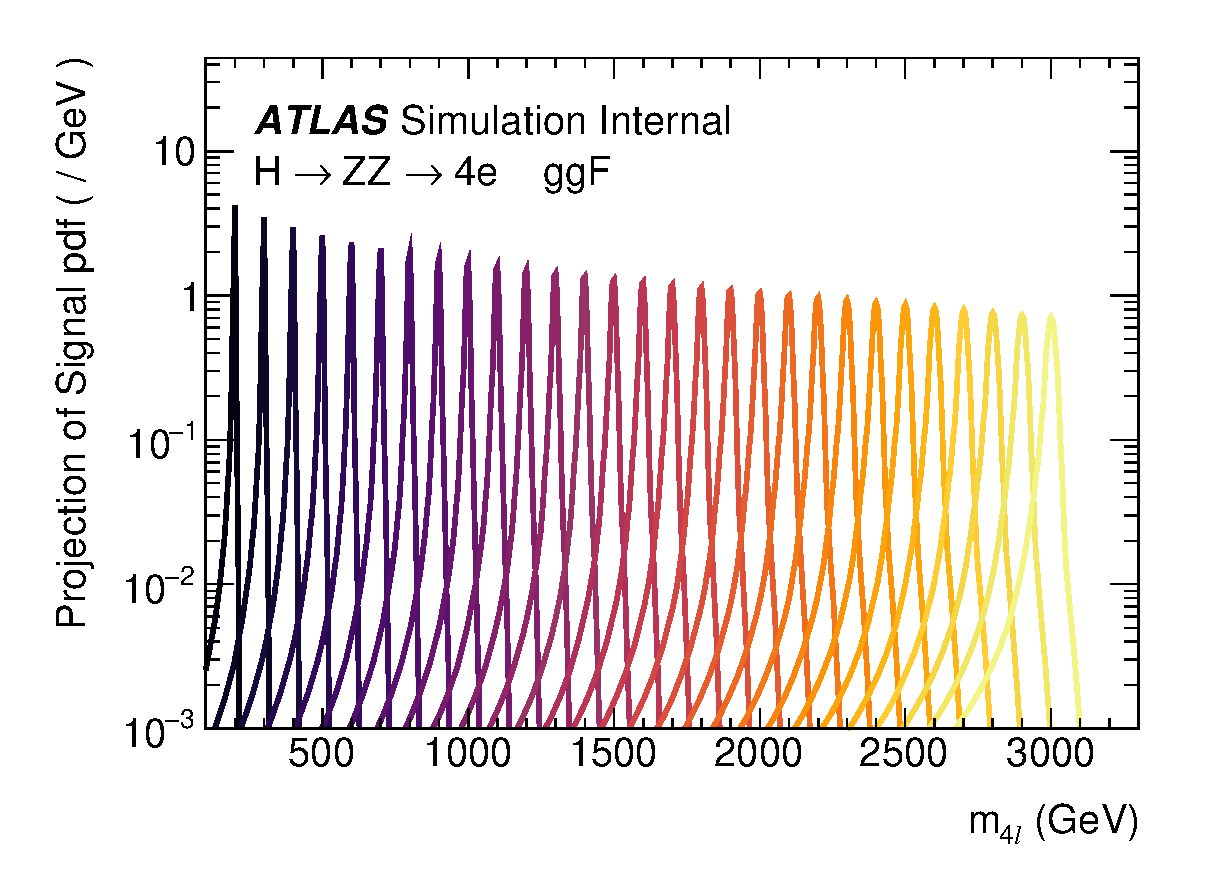
\includegraphics[width=0.32\textwidth]{figures/HMHZZ/signal/ggf_multipeakplot_4e.eps}
    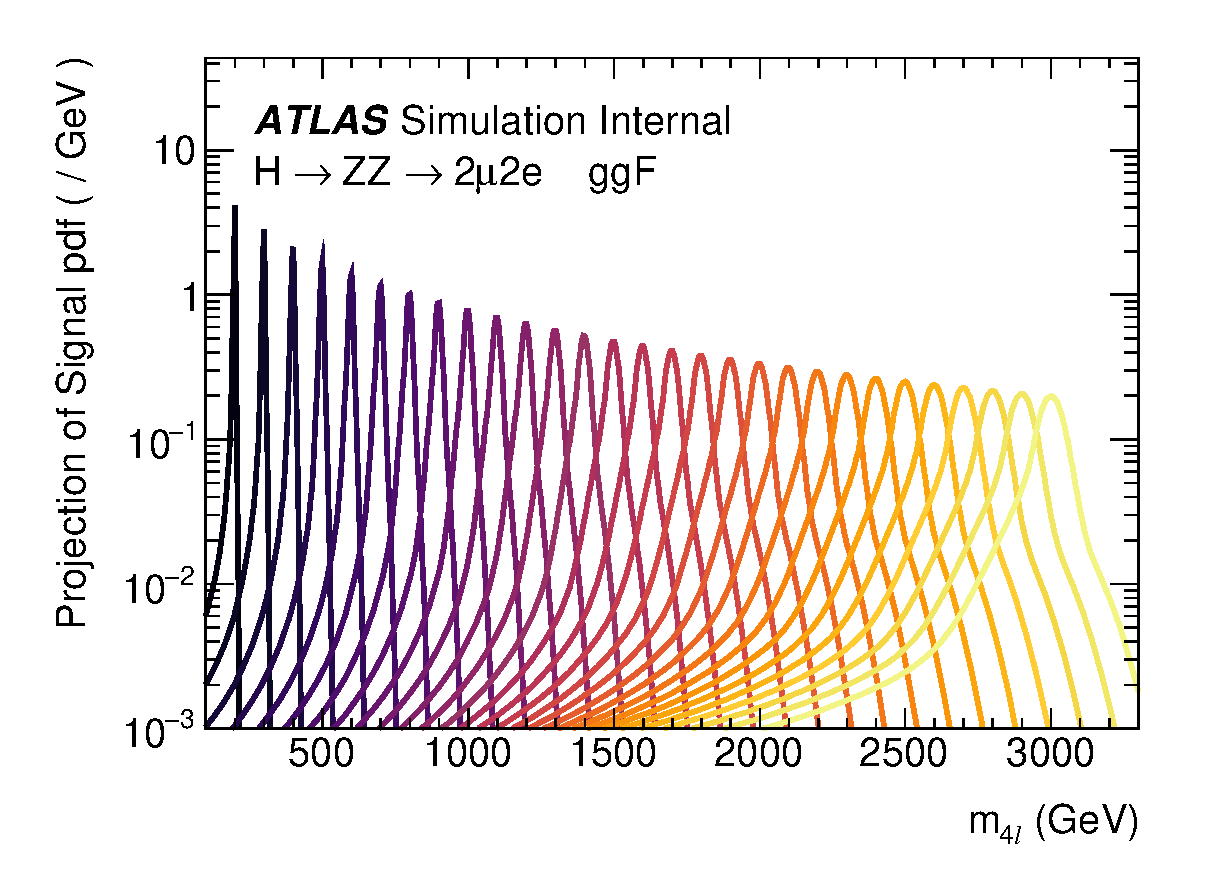
\includegraphics[width=0.32\textwidth]{figures/HMHZZ/signal/ggf_multipeakplot_2mu2e.eps}
    \caption{The final signal shapes for the ggF production mode, interpolated from the polynomial fit parameters.}
    \label{fig:ggf_multipeak}
\end{figure}

\subsection{Modelling of large-width signal}


